\documentclass[11pt]{article}

\usepackage{maiacustom}

\begin{document}

\psettitle{Astronomy Question Bank}

These questions were carefully written or selected to prepare students for the astronomy team selection process in Brazil. Some questions are not original; those are marked with () before the statement. The question-bank template is the same one used by Professor Kevin Zhou. His work is invaluable, and many ideas in this set can be found in his handouts.

% \begin{psidea}{Idea title}{}
% Idea
% \end{psidea}

% \begin{psexample}{Example title}{}
% Example
% \end{psexample}

% \begin{pssolution*}{}{}
% Solution
% \end{pssolution*}

% \begin{psremark*}{Remark title}{}
% Remark
% \end{psremark*}
\section{Positional Astronomy}

\pts{5} % problem of the week 114
\begin{pproblem} After getting lost on a voyage, you and Professor Klafke are shipwrecked on an island and find the following sundial:
    \begin{figure}[H]
        \centering
        \includegraphics[width=0.5\linewidth]{imagens/q6.jpg}
        \caption{Sundial}
    \end{figure}
    It is now your task to discover properties of the sundial.
    \begin{enumerate}[label=\textbf{\alph*)}]
        \item In which hemisphere did you find yourselves? How did you reach that conclusion?
        \item After several weeks on the island, you notice that the sundial's shadow seems to follow a straight line. Letting \(\phi\) be the latitude at which you found yourselves, determine the Sun's declination on that day and explain why this happens on only \(2\) days of the year.
        \item Prove that, when the Sun has the declination found above, the shadow follows a straight line. This can be done by the following steps:
        \begin{enumerate}[label=\roman*)]
            \item Determine the orientation of the line and explain why it must have that orientation;
            \item Determine the length of the shadow for a given position of the Sun in alt-azimuth coordinates;
            \item Derive a relation between altitude and azimuth, given that the tip of the shadow lies on the line;
            \item Determine a constant quantity and show that it is constant for every position of the Sun on that day.
        \end{enumerate}
    \end{enumerate}


\begin{pssolution*}{}{}
    \begin{alternativas}
        \item From the figure, we can see that the markings on the left correspond to the morning hours. The Sun is therefore rising on the right, so that its shadow falls on the left. From these arguments, the cardinal point \textit{East} lies on the right and \textit{West} on the right. A vertical sundial always has its gnomon pointed toward the non-elevated celestial pole. Since this one points \textit{south}, we conclude that the sundial is in the \(\boxed{\textit{Northern Hemisphere}}\).

        \item This happens only at the equinoxes, when \(\delta_\odot = 0\).

        \item Following the steps in the statement, 
        \begin{enumerate}[label=\roman*)]
            \item Since \(\delta_\odot=0\), the sky moves exactly from east to west, 
            \item If the gnomon has length \(L\) and the Sun is at an altitude \(h\), geometry gives the shadow length \(l\) as \(l=\frac{L}{\tan h}\).
            \item Consider the following figure, 
            \begin{figure}[H]
                \centering
                \includegraphics[width=0.66\linewidth]{imagens/retarelogiosolvert.png}
                \caption{Diagram of the imaginary line}
            \end{figure}
        \end{enumerate}

        The distance from the center of the sundial to the shadow is

        \[x = l\sin (A-90^{\circ})\equiv l\sin a = L\frac{\sin a}{\tan h}\]

        We now want to prove that this quantity is constant.

        \item Consider the following triangle: 
        
        \begin{figure}[H]
            \centering
            \includegraphics[width=0.5\linewidth]{imagens/trigesf1.jpg}
            \caption{Sun on the equator}
        \end{figure}

        Using the four-parts formula, 

        \[\cot(90^\circ -\phi)\sin(90^{\circ})+\cos a \cos(90) = \cot h \sin a\]

        Simplifying, we have 

        \[\frac{\sin a}{\tan h } = \tan {\phi}\]

        which is constant. Our condition is therefore proved.

    \end{alternativas}
\end{pssolution*}
\end{pproblem}

\pts{5}
\begin{pproblem} (Adapted from T1 - 2024)
    The equation of time is the difference between the right ascension of the mean Sun and the right ascension of the true Sun. With that in mind, let us calculate some of its properties.
    \begin{alternativas}
        \item Find an expression for the equation of time, neglecting Earth's eccentricity, i.e.: the Sun moving at constant speed along the ecliptic. Leave your answer in terms of the time since the March equinox \(T_M\), Earth's period \(T\), and the obliquity of the ecliptic \(\epsilon\).
        \item Now, taking Earth's eccentricity into account, the equation of time has the form:
        \[E.T. = -2e \cdot \sin(k_1 \cdot M) + \tan^2 \left( \frac{\epsilon}{2} \right) \cdot \sin\left( k_2 \cdot (M + \lambda_P) \right)\]
        where \(M\) is the mean anomaly, \(\lambda_P\) the ecliptic longitude of periapsis, and \(e\) Earth's eccentricity. Determine the constants \(k_1\) and \(k_2\). Think about the symmetries involving each term of the equation.
        \\
        The aim of the question is now to find the Sun's declination at the node of the analemma. See the following figure:
        \begin{figure}[H]
            \centering
            \includegraphics[width=0.7\textwidth]{imagens/q16.png}
            \caption{Analemma diagram}
        \end{figure}
        The node is the point at which the path crosses itself.
        \item For small values of the Sun's declination, obtain a formula for it in terms of \(M\), \(\lambda_P\), and \(\epsilon\). Also assume that the eccentricity and the orbital inclination are sufficiently small.
        \item Find the two mean anomalies that have the same declination and the same \(E.T.\).
        \item Find the value of the solar declination at the node.
    \end{alternativas}

\begin{pssolution*}{}{ }
    \begin{alternativas}
        \item The equation of time is given by
        
        \[E.T. = \alpha_M - \alpha_V\]

        where \(\alpha_M\) is the right ascension of the mean Sun, i.e.: a ``fictitious Sun'' that moves along the celestial equator at constant speed, and \(\alpha_V\) is the right ascension of the true Sun.

        Consider the following spherical triangle

        INSERT image

        First, both the true Sun and the mean Sun have constant and equal angular speeds \(\omega_\odot = 2\pi/T\), so \(\alpha_M=\omega_\odot T_M\).

        Using the four-parts formula

        \[\cot \pi/2 \sin\epsilon + \cos\epsilon\cos\alpha_V=\cot(\omega_\odot T_M)\sin\alpha_V\]

        Since \(\cot\pi/2 =0\), we obtain

        \[\alpha_V = \tan^{-1}(\cos\epsilon\tan(\omega_\odot T_M))\]

        Note that when \(\epsilon = 0\), \(\alpha_V = \alpha_M\), as expected.

        Finally, returning to the definition of the equation of time

        \[\boxed{E.T. = \tan^{-1}\left(\cos\epsilon\tan\left(\frac{2\pi}{T} T_M\right)\right) - \frac{2\pi}{T}T_M}\]

        \item To solve this problem, consider the symmetries. For an elliptical orbit, the only symmetry is about the major axis. Once the obliquity of the ecliptic is included, there are two possible symmetries, about the line of the solstices and about the line of the equinoxes. It is therefore reasonable to expect that the sinusoid tied to the orbital eccentricity has one period per year, while the one tied to the obliquity of the ecliptic has two periods per year. Thus \(\boxed{k_1=1, \ k_2 = 2}\)
        
        \item Returning to the previous spherical triangle and using the law of sines, we have
        
        \[\frac{\sin\delta_\odot}{\sin\epsilon} = \sin\lambda\]

        where \(\lambda \) is the ecliptic longitude of the Sun. Using \(\sin\theta \approx \theta\) for small angles, we have

        \[\delta_\odot = \epsilon\sin\lambda\]

        Neglecting the eccentricity, \(\lambda = \lambda_P + M\), so

        \[\boxed{\delta_\odot = \epsilon\sin(\lambda_P + M)}\]

        \item The condition for two mean anomalies to have the same equation of time is 
        \[\sin(M_1+\lambda_P) = \sin(M_2+\lambda_P)\]

        Using \(\sin\theta = \sin(\pi-\theta)\), we have

        \[\boxed{M_2 =\pi -M_1-2\lambda_P}\]

        \item Equating the equations of time
        
        \[-2e\sin(M_1) + \tan^2 \left( \frac{\epsilon}{2} \right)\sin\left(2(M_1 + \lambda_P) \right) = -2e\sin(M_2) + \tan^2 \left( \frac{\epsilon}{2} \right)\sin\left(2(M_2 + \lambda_P) \right)\]

        Substituting \(M_2\)  

        \[-2e\sin(M_1) + \tan^2 \left( \frac{\epsilon}{2} \right)\sin\left(2(M_1 + \lambda_P) \right) = -2e\sin(M_1+2\lambda_P) - \tan^2 \left( \frac{\epsilon}{2} \right)\sin\left(2M_1 + 2\lambda_P \right)\]

        \[\tan^2 \left( \frac{\epsilon}{2} \right)\sin(2M_1+2\lambda_P) = e(\sin M_1 - \sin(M_1+\lambda_P))\]

        Using the double-angle formula for sine and the prosthaphaeresis formulas:

        \[\tan^2\left(\frac{\epsilon}{2}\right)\sin(M_1+\lambda_P)\cos(M_1+\lambda_P) = -e\sin\lambda_P\cos(M_1+\lambda_P)\]

        \[\sin(M_1+\lambda_P) = -\frac{e\sin\lambda_P}{\tan^2\left(\frac{\epsilon}{2}\right)}\approx -\frac{4e\sin\lambda_P}{\epsilon^2}\]

        Finally, substituting into the declination formula:

        \[\boxed{\delta_\odot \approx -\frac{4e\sin\lambda_P}{\epsilon}}\]
    \end{alternativas}
\end{pssolution*}
\end{pproblem}

    
\pts{5}
    \begin{pproblem}
        Porílio, after a long day of classes at ITA, on the summer solstice (\(\phi = 23^\circ 11' S, \ \lambda = 45^\circ 53' W\)) wants to watch the sunset. On the day in question, the equation of time is \(E.T. = -3\) minutes. Porílio does not want to miss the Sun under any circumstances and starts running so that the (center of the) Sun stays on the horizon.
    
        \begin{alternativas}
            \item São José dos Campos follows Brasília time (UTC-3h). At what civil time should Porílio start his run?
            \item If Porílio runs toward one of the geographic poles, what should his initial speed be?
            \item If Porílio decides to climb a mountain of inclination \(i = 30^\circ\) at a constant speed \(v = 1\) m/s, what is the longest time for which Porílio can keep the Sun above the horizon?
            \textbf{Hint: } Small-angle approximations may be useful.
        \end{alternativas}

\begin{pssolution*}{}{ }
    \begin{alternativas}
        \item To find the rising or setting time of a star, we need its hour angle at the moment it rises. Consider the following spherical triangle, 
        
        \begin{figure}[H]
            \centering
            \includegraphics[width=0.8\linewidth]{imagens/trigangulohorario.png}
            \caption{Diagram of the Sun on the horizon}
        \end{figure}

        When the Sun is on the horizon, \(h = 0\). Because this is the summer solstice (in the Southern Hemisphere), \(\delta = -23^\circ 47'\). Using the law of cosines together with \(\sin(90 - \theta) = \cos(\theta)\) and \(\cos(90 - \theta) = \sin(\theta)\), we have 

        \[\sin h = \sin\phi\sin\delta + \cos\phi\cos\delta\cos H\]

        Solving for \(H\), and using \(\sin h = \sin 0^\circ = 0\), 

        \[\cos H = -\tan\phi\tan\delta\]

        Solving, we obtain \(H = 100.72^\circ = 6^h 42^m 52^s\)

        The time of sunset is given by \(TSL = 12 + H = 18^h 42^m 52^s\).

        Using \(TC = TSL + (\lambda_{\text{zone}} - \lambda_{\text{local}})/15 - E.T.\), we obtain 

        \[\boxed{TC = 18^h 49^m 20^s}\]

        \item Porílio must run toward the South Celestial Pole, since the Sun's declination is negative. To find his initial speed, differentiate the law of cosines with respect to time at \(h = 0\).
        \[\frac{d\cos H}{dt} = -\tan\delta \frac{d\tan\phi}{dt}\]

        Using the chain rule, 

        \[-\sin H \dot{H} = -\frac{\tan\delta}{\cos^2\phi}\dot{\phi}\]

        where \(\dot{a} = \frac{da}{dt}\). Isolating \(\dot{\phi}\), 

        \[\dot{\phi} = \frac{\cos^2\phi\sin H}{\tan\delta}\dot{H}\]

        The hour angle changes at \(360^\circ / 24^h = 15^\circ / 1^h\). Solving for \(\dot{\phi}\), 

        \[\dot{\phi} = -28.68^\circ/h = -1.39 \cdot 10^{-4} \text{ rad/s}\]

        The sign of \(\dot{\phi}\) only means that he is moving toward the South Pole. Using 

        \[\dot{\phi} = \frac{v}{R_\oplus}\]

        we arrive at \(v = R_\oplus|\dot{\phi}|\),
        
        \[\boxed{v \approx 885 \text{ m/s}}\]

        \item We now use the horizon angle. Consider the following figure, 
            \begin{figure}[H]
                \centering
                \includegraphics[width=0.90\linewidth]{imagens/angulohorizonte.png}
                \caption{Source: Magna notes}
            \end{figure}

            The angle \(\theta\) is given by

            \[\cos\theta = \frac{R_T}{R_T + h}\]

            Since \(h \ll R_T\), set \(x = h / R_T\) and use the approximations for \(x \ll 1\).

            \[\cos\theta = \left(\frac{R_T + h}{R_T}\right)^{-1} = \left(1 + \frac{h}{R_T}\right)^{-1} \approx 1 - \frac{h}{R_T}\]

            Since \(\theta\) is small, use the second-order Taylor expansion 

            \[f(x) \approx \sum \frac{f^{(n)}(a) x^n}{n!}\]

            where \(f^{(n)}(x)\) is the \(n\)th derivative of \(f(x)\). Expanding about \(a = 0\), 

            \[\cos\theta \approx 1 - \frac{\theta^2}{2}\]

            Equating the two expressions, 

            \[1 - \frac{\theta^2}{2} = 1 - \frac{h}{R_T} \rightarrow \theta = \sqrt{\frac{2h}{R_T}}\]

            To find how long the Sun stays above the horizon, compute the time over which the Sun's apparent altitude is offset by the angle \(\theta\), so that the Sun remains on the horizon. The law of cosines then becomes 

            \[\sin\theta = \sin\phi\sin\delta + \cos\phi\cos\delta\cos H\]

            Using \(\sin\theta \approx \theta\), 

            \[\theta = \sin\phi\sin\delta + \cos\phi\cos\delta\cos H\]

            Differentiate both sides with respect to time. (Here \(\dot{\phi}\) is neglected, because Porílio's speed is very small.)

            \[\frac{d\theta}{dt} = -\cos\phi\cos\delta\sin H \dot{H}\]

            To differentiate \(\theta\) with respect to time, note that \(h(t) = v t \sin i\).

            \[\frac{d\theta}{dt} = \sqrt{\frac{2v\sin i }{R_T}}\frac{d}{dt}\sqrt{t} = \sqrt{\frac{v\sin i}{2 R_T t}}\]

            Equating the two expressions, 

            \[\frac{v\sin i}{2R_T t} = (\cos\phi\cos\delta\sin H \dot{H})^2\]

            \[t = \frac{v\sin i}{2R_T(\cos\phi\cos\delta\sin H \dot{H})^2}\]

            \[\boxed{t \approx 10.82 \text{ s}}\]

    \end{alternativas}
    
\end{pssolution*}
\end{pproblem}



\pts{3}
\begin{pproblem}
    Mauí, a renowned astronomer, wants to spend his year-end vacation in Sergipe \((10^\circ \ 54'\ 33'' S, \ 37^\circ 4'29'' W)\) and wants to know the rising time of one of his favorite stars, All Kaf al Dij Ma \Romannum{3} \((\delta = +10^\circ \ 56'\ 58'', \ \alpha = 2h \ 58m \ 43s\)), and needs your help to calculate its rising time in the following situations:
    
    \begin{alternativas}
        \item Calculate the rising time of All Kaf al Dij Ma \Romannum{3} at the December solstice.
        \item How long will the star spend above the horizon?
        \item Estimate the length of time during which the star is visible.
    \end{alternativas}

\begin{pssolution*}{}{ }
    \begin{alternativas}
        \item As seen above, the hour angle at which a star rises is given by 

        \[\cos H = - \tan \delta \tan \phi \rightarrow H = \]

        The time follows from 

        \[TSL = \alpha + H\]

        which gives \(\boxed{TSL = \text{result}}\)

        \item The time the star spends above the horizon is 
        
        \[\Delta t = 2 H = \]

        \item At the summer solstice, \(\delta_\odot = -23.47\), so the Sun's hour angle is \(H_\odot = -\tan\delta_\odot \tan\phi = \). That is, the time for which the Sun is visible is \(\delta t_\odot = \). A valid estimate of the time for which the star is visible is 
        \[\Delta t = 2 (H - H_\odot)\]

        These are the intervals during which the star is above the horizon while the Sun is not: 
       
        \[\boxed{\Delta t = \text{result}}\]
    \end{alternativas}
\end{pssolution*}
\end{pproblem}


\pts{4}
\begin{pproblem}(Lucas Cavalcante - \href{https://noic.com.br/olimpiadas/astronomia/problemas-da-semana/astronomia-semana-111/}{Week 111})
    Consider a horizontal coordinate system in which azimuth \(0\) corresponds to the north cardinal point. One asteroid was observed at altitudes \(h_1\) and \(h_2\) and azimuths \(A_1\) and \(A_2\), while another asteroid was observed at the coordinates \(h_3\), \(h_4\), \(A_3\), and \(A_4\). Find the coordinates of the points where the asteroids meet.
    
    \begin{psidea}{Einstein notation}{}
    While solving this problem, I will use Einstein notation. It is a tool from physics that makes vector calculations easier. In ordinary notation, a vector is written as
    \[\mathbf{a} = (a_1 \hat{\mathbf{e}}_1, \ a_2 \hat{\mathbf{e}}_2, \ a_3 \hat{\mathbf{e}}_3)\]
    In Einstein notation, this is replaced by:
    \[\mathbf{a} = a_i \hat{\mathbf{e}}_i\]
    Repeated indices indicate a sum (\(a_i \hat{\mathbf{e}}_i = a_1 \hat{\mathbf{e}}_1 + a_2 \hat{\mathbf{e}}_2 + a_3 \hat{\mathbf{e}}_3 + ...\))
    
    The scalar product of two vectors, in Einstein notation, is defined by:
    \[\mathbf{a}\cdot \mathbf{b} = a_i b_j \delta_{ij}\]
    where \(\delta_{ij}\) is the \textit{Kronecker delta}, defined by:
    \[\delta_{ij} = \left \{ \begin{matrix} 0, & \mbox{if } i \ne j \\ 
                                            1, & \mbox{if } i = j\end{matrix} \right.\]
    
    Thus, \(\mathbf{a}\cdot \mathbf{b} = a_i b_i \equiv a_1 b_1 + a_2 b_2 + a_3 b_3\)

    For the cross product, we have:
        \[
        \mathbf{a} \times \mathbf{b} = a_i b_j \Epsilon_{ijk} \hat{\mathbf{e}}_k
        \]
        Here, \(\Epsilon_{ijk}\) is called the \textit{Levi-Civita tensor}, or Levi-Civita symbol, and is defined as:
    
        \[
        \Epsilon_{ijk} = 
        \begin{cases} 
        +1 & \text{if } (i, j, k) \text{ is an even permutation of } (1, 2, 3), \\
        -1 & \text{if } (i, j, k) \text{ is an odd permutation of } (1, 2, 3), \\
        0 & \text{if two or more indices are equal}.
        \end{cases}
        \]

        For example, \(\Epsilon_{123} = \Epsilon_{312} = \Epsilon_{231} = 1\) and \(\Epsilon_{132} = \Epsilon_{213} = \Epsilon_{321} = -1\).
        Explicitly 
        \[\mathbf{a} \times \mathbf{b} = (a_2 b_3 - a_3 b_2) \hat{\mathbf{e}}_1 + (a_3 b_1 - a_1 b_3) \hat{\mathbf{e}}_2 + (a_1 b_2 - a_2 b_1) \hat{\mathbf{e}}_3\]
    \end{psidea}
\begin{pssolution*}{}{}
    To solve this problem we use two central facts about vectors. Given two vectors $\mathbf A$ and $\mathbf B$, $\mathbf A \cdot \mathbf B$ lies in the plane formed by $\mathbf A$ and $\mathbf B$, while $\mathbf A \times \mathbf B$ is perpendicular to that plane. Let $\mathbf r_1$ and $\mathbf r_2$ be two vectors giving the positions of the first asteroid, and $\mathbf r_3$ and $\mathbf r_4$ the two position vectors of the second asteroid. The orbit of the first asteroid lies in the plane of $\mathbf r_1 \cdot \mathbf r_2$, and the orbit of the second asteroid lies in the plane of $\mathbf r_3 \cdot \mathbf r_4$. What actually solves the problem is the cross product, because it is perpendicular to the orbit. The following figure makes this easier to see:

    \begin{figure}[H]
        \centering
        \includegraphics[width=0.8\linewidth]{imagens/orbitas3.png}
        \caption{Diagram of the orbits and of the cross products}
    \end{figure}

    Going one step further, the operation \((\mathbf r_1 \times \mathbf r_2)\times(\mathbf r_3 \times \mathbf r_4)\) produces a vector perpendicular both to \(\mathbf r_1\times \mathbf r_2\) and to \(\mathbf r_3\times \mathbf r_4\). That vector \textbf{necessarily} passes through the point the two orbits have in common.

    \begin{figure}[H]
        \centering
        \includegraphics[width=0.8\linewidth]{imagens/orbitas4.png}
        \caption{Meeting point}
    \end{figure}

    By symmetry, $(\mathbf r_3\times \mathbf r_4)\times(\mathbf r_1\times \mathbf r_2)\equiv - (\mathbf r_1 \times \mathbf r_2)\times (\mathbf r_3 \times \mathbf r_4)$ is also a meeting point. We now compute this vector.

    To convert the vector specified by $h_i$ and $A_i$ (spherical coordinates) into $x_i$, $y_i$, and $z_i$, 

    $$\mathbf r_i = (\cos h_i\cos A_i, \ \cos h_i\sin A_i, \ \sin h_i)$$

    where the axes are oriented so that $x$ points north and $z$ points toward the zenith. Carrying out the calculation in Einstein notation, 

    \[(\mathbf r_1 \times \mathbf r_2)\times(\mathbf r_3 \times \mathbf r_4) = (r_{1,i}r_{2,j}\varepsilon_{i,j,k}\mathbf{\hat{e}}_k)\times(r_{3,m}r_{4,n}\varepsilon_{m,n,o}\mathbf{\hat{e}}_o)\]

    Simplifying, 

    \[= \varepsilon_{i,j,k}\varepsilon_{m,n,o}r_{1,i}r_{2,j}r_{3,m}r_{4,n}(\varepsilon_{k,o,p}\mathbf{\hat{e}}_p)\]
    \[= \varepsilon_{i,j,k}\varepsilon_{m,n,o}\varepsilon_{k,o,p}r_{1,i}r_{2,j}r_{3,m}r_{4,n}\mathbf{\hat{e}}_p\]

    To simplify further, use the identity 

    \[\varepsilon_{a,b,c}\varepsilon_{a,d,e} = \delta_{b,d}\delta_{c,e}-\delta_{b,e}\delta_{c,d}\]

    The expression becomes 

    \[\varepsilon_{m,n,o}r_{3,m}r_{4,n}(\delta_{io}\delta_{jp}-\delta_{ip}\delta_{jo})r_{1,i}r_{2,j}\mathbf{\hat e}_p\]
    
    Contracting the Kronecker deltas reduces it to 

    \[(\varepsilon_{m,n,o}r_{3,m}r_{4,n}r_{1,o}r_{2,p}-\varepsilon_{m,n,o}r_{3,m}r_{4,n}r_{1,p}r_{2,o})\mathbf{\hat e}_p\]

    At first glance this looks forbidding, maybe even worse than the vector expression, but with practice the notation reads more smoothly and more directly. After a great deal of grinding algebra, we arrive at 

    \[\boxed{(\mathbf r_1 \times \mathbf r_2)\times(\mathbf r_3 \times \mathbf r_4) = T_1\mathbf r_2 - T+2\mathbf r_1}\]

    where

    \[
    \begin{aligned}
    T_1 &= 
    \cos h_1 \cos h_3 \sin h_4 \sin(A_3 - A_1)
    + \cos h_1 \cos h_4 \sin h_3 \sin(A_1 - A_4) \\
    &\quad + \sin h_1 \cos h_3 \cos h_4 \sin(A_4 - A_3)
    \end{aligned}
    \]

    \[
    \begin{aligned}
    T_2 &=
    \cos h_2 \cos h_3 \sin h_4 \sin(A_3 - A_2)
    + \cos h_2 \cos h_4 \sin h_3 \sin(A_2 - A_4) \\
    &\quad + \sin h_2 \cos h_3 \cos h_4 \sin(A_4 - A_3)
    \end{aligned}
    \]

    Reaching a closed formula is interesting but very laborious. This approach is nevertheless well suited to numerical values, and it turns difficult problems into much simpler ones.
\end{pssolution*}
\end{pproblem}


\pts{5}
\begin{pproblem} (Problem set \(1\) - Vinhedo 2024) Consider a sundial consisting of a vertical dial
    and a gnomon, as shown in the figure.
    \begin{figure}[H]
        \centering
        \includegraphics{imagens/q20.png}
        \caption{Sundial diagram.}
    \end{figure}
    \begin{alternativas}
        \item Suppose a vertical sundial whose gnomon is correctly pointed south.
        Let \(\phi\) be the observer's latitude, \(H\) the Sun's hour angle, and \(\delta\) the solar declination. Determine
        the relation between \(\theta\) and \(\gamma\) in terms of these variables.
        
        \item From the previous item, what must \(\theta\) be for the sundial to work throughout the year?

        \item Using the correct value of \(\theta\), determine the relation between \(\gamma\) and \(H\), in terms of \(\phi\) only.
    \end{alternativas}
\end{pproblem}

\pts{2} 
\begin{pproblem}
    What is the smallest height a giant (who lives a VERY long time), located at the South Pole, must have in order to see every star in the sky?

    \begin{pssolution*}
        The angle below the horizon that the giant can see is given by 
    
        \[\cos\theta = \frac{R_\oplus}{R_\oplus + H}\]
    
        where \(H\) is the giant's height. Because of the precession of the equinoxes, the south pole will lie \(23.47^\circ\) above the ecliptic. The horizon angle must therefore be \(\theta = 90^\circ - 23.47^\circ = 66.53^\circ\). Solving for \(H\), 
    
        \[\boxed{H = R_\oplus\left(\frac{1}{\cos\theta}-1\right) \approx 9.62\cdot 10^6\text{ m}}\]
    \end{pssolution*}
\end{pproblem}    


\pts{3}
\begin{pproblem}
    Toleduardo wants to watch the sunset, but he spent too long at SorveterITA. Toleduardo is a \textit{Just in time} man and wants to know how long the sunset will last, so that he can be late at his leisure. Given that Toleduardo only goes to SorveterITA on March 21 or September 22, calculate the duration of the sunset at SorveterITA.
    \\
    \textbf{Data: } Latitude of SorveterITA \(\phi = 23^\circ \ 10' \ 45''S, \ \ \lambda = 45^\circ 53' 14''W\).
\end{pproblem}
\begin{pssolution*}{}{}
    
    To work out this solution, take the astronomical triangle for the Sun and write an equation for its hour angle.

    \[\sin h = \sin\delta\sin\phi + \cos\delta\cos\phi\cos H\] 

    Differentiating with respect to time, 

    \[\dot h \cos h = -\dot H \cos\delta\cos\phi \sin H\]

    At sunset, 

    \[H_0 = \cos^{-1}\left(-\tan\delta\tan\phi\right)\]

    Near \(h=0\), 

    \[\left. \frac{dh}{dt}\right|_{h=0} = -\dot H \cos\delta\cos\phi\sin H_0\]

    On the day in question, \(\delta = 0\) (the equinoxes), so \(H_0 = 6h\)

    \[\left. \frac{dh}{dt}\right|_{h=0} - \dot{H}\cos\phi\sin H_0\]

    Note that \(\dot H = 15^{\circ}/h\). Solving for \(dt\), 
    
    \[dt \approx \frac{-dh}{\dot{H}\cos\phi \sin H_0}\]

    Integrating and using \(\sin H_0 = 1 \), 

    \[\Delta t \approx -\frac{1}{\dot H \cos \phi}\int_{\theta\odot}^{-\theta\odot}dh\]

    \[\Delta t \approx \frac{2\theta_\odot}{\dot H \cos \phi}\]

    \[\boxed{\Delta t \approx 4^m38^s}\]
\end{pssolution*}


\pts{3}
\begin{pproblem} (Problem set 2 - Vinhedo 2021)
    In February 2015, the Moon began a cycle of monthly occultations of Aldebaran ($\alpha$ Tau). That is, every month the Moon passed in front of Aldebaran for an observer on Earth. Note that these occultations did not necessarily occur for observers at the same location every month. 

    Calculate the date (month and year) when this cycle of monthly occultations ends. Assume that the Moon's orbit is circular.

    \subsection*{Data:}

    \begin{itemize}
        \item Ecliptic latitude of Aldebaran = $5.47^\circ$
        \item Nodal precession period of the Moon = 18.6 years
    \end{itemize}
\end{pproblem}

\begin{pssolution*}{}{}
    The Moon's nodal precession makes the nodes of the lunar orbit on the ecliptic rotate with a period of 18.6 years. Over that period, the Moon's ecliptic latitude as it crosses the meridian of Aldebaran's ecliptic longitude therefore ranges from $-5.15^\circ$ to $5.15^\circ$ (the lunar orbit is inclined by $\gamma=5.15^\circ$ to the ecliptic). 
    
    The first step is to find the maximum ecliptic longitude (or the one of smallest absolute value) at which the Moon occults Aldebaran. From the following figure:

    \begin{figure}[H]
        \centering
        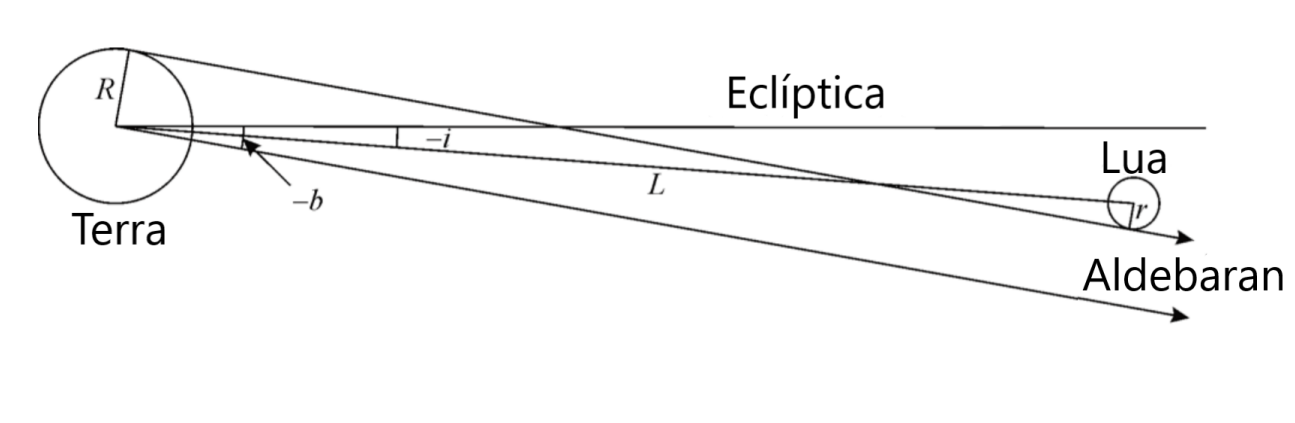
\includegraphics[width=0.99\linewidth]{imagens/lua-aldebaran.png}
    \end{figure}

    Basic trigonometry gives

    \[-b-(-i) = \sin^{-1}\left(\frac{R+r}{L}\right)\]

    \[i = b+\sin^{-1}\left(\frac{R+r}{L}\right)\]

    Substituting, we obtain \(i\approx -4.26^\circ\). We next need the angle that covers every point at which the Moon's ecliptic latitude exceeds \(|i|\). Use the following spherical triangles:

    \begin{figure}[H]
        \centering
        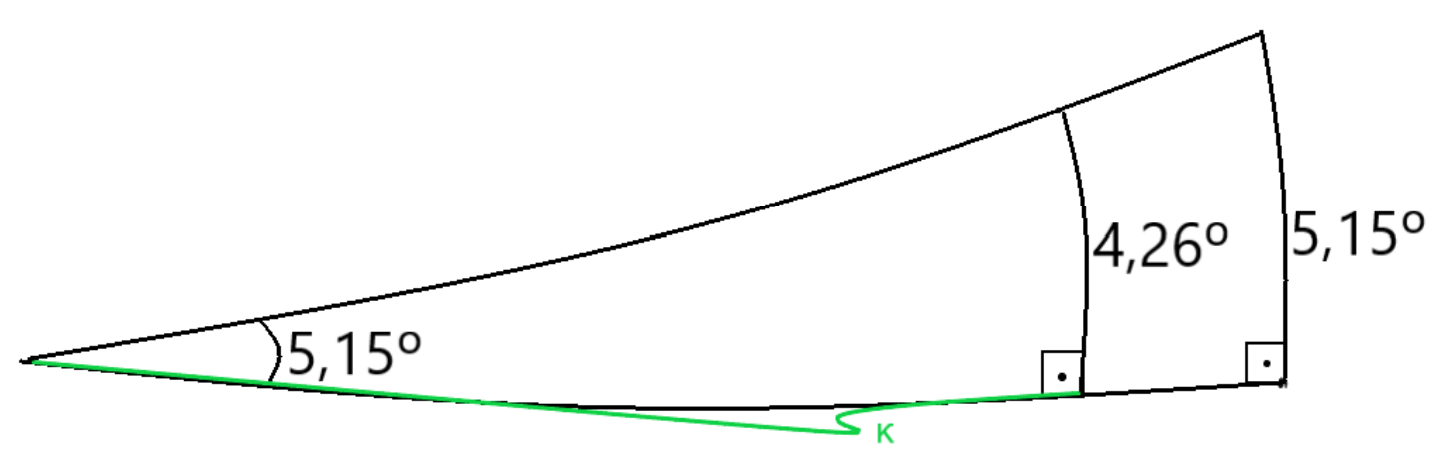
\includegraphics[width=0.99\linewidth]{imagens/lua-aldebaran2.png}
    \end{figure}

    The four-parts formula determines $\kappa$, 

    \[\cos(\kappa)\cos(90^\circ) = \sin(\kappa)\cot (4.26^\circ)-\sin(90^\circ)\cot(5.15^\circ)\]

    \[\sin(\kappa)=\frac{\tan(4.26^\circ)}{\tan(5.15^\circ)}\]

    \[\kappa = 55.74^\circ \]

    The range of ecliptic longitudes over which the Moon can occult Aldebaran is then

    \[\Gamma = 2(90^\circ-\kappa) = 68.52^\circ \]

    so the time interval is 

    \[\Delta t = \frac{\Gamma}{360^\circ}T \]

    \[\boxed{\Delta t = 3.54 \text{ years}}\]

    Since the occultations began in February 2015, 

    \[\text{February 2015} + 3.54\text{ years} = \text{August 2018}\]

    \(\therefore\) The occultation cycle ends in \(\boxed{\text{August 2018}}\).

\end{pssolution*}



\pts{4}
\begin{pproblem} (Problem set 2 - Vinhedo 2021)
    Miguel lives on an isolated island in the South Pacific Ocean, at longitude
    $\lambda = 176^{\circ}09^{\prime}137.7^{\prime\prime}\text{W}$. Over the year, the place where the Sun rises, as seen by Miguel, varies by $\Delta A = 67^{\circ}03^{\prime}81^{\prime\prime}$ along the horizon. For the first two items, neglect atmospheric refraction. With this information, find:

    \begin{alternativas}
        \item The latitude $\phi$ and the name of the island. (Consult Google Earth or similar software)
        \item The range of times at which the Sun rises on the island, given the peculiar time zone $UT + 12\frac{3}{4}$.
        \item Taking atmospheric refraction into account, would the length of the interval in the previous item decrease, increase, or stay constant?
    \end{alternativas}

\begin{pssolution*}{}{}
    \begin{alternativas}
        \item Consider the sketch of the situation, 
        
        \begin{figure}[H]
            \centering
            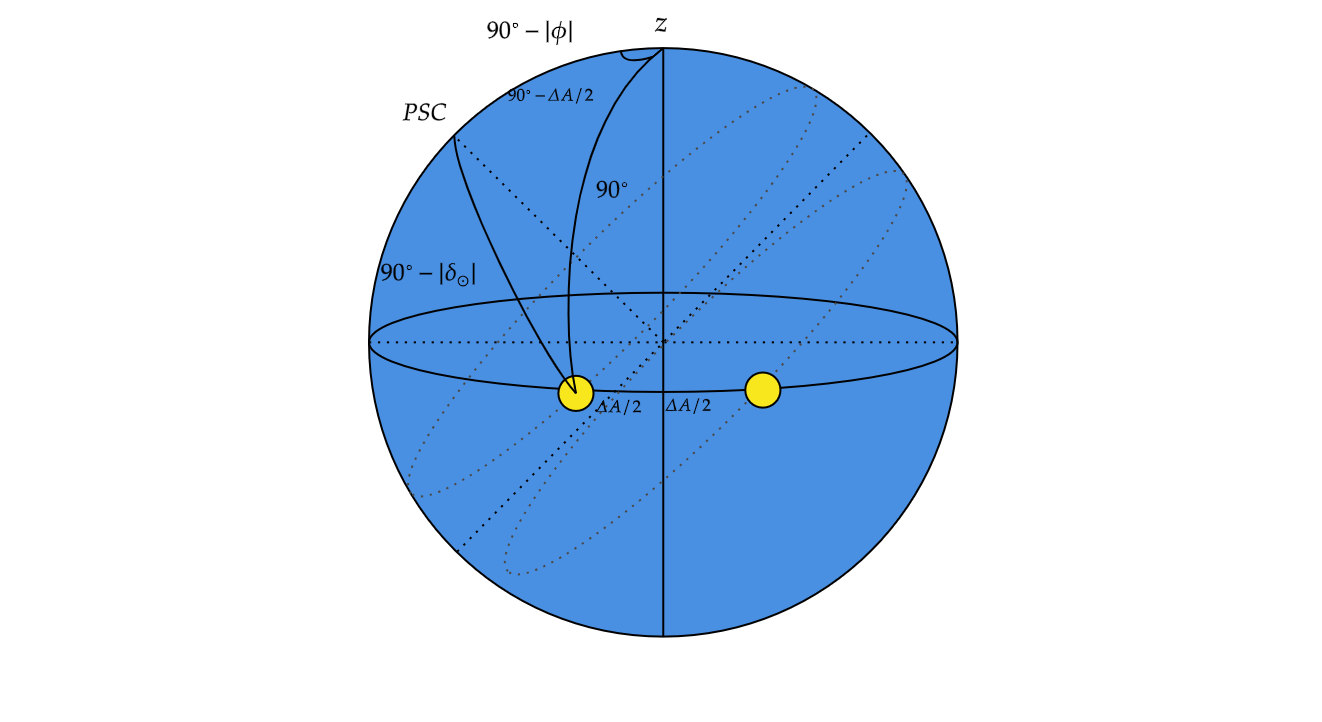
\includegraphics[width=0.99\linewidth]{imagens/sol-ilha.png}
        \end{figure}

        Using the law of cosines, 

        \[\cos(90^\circ-|\delta_\odot|) = \cos(90^\circ)\cos(^\circ-|\phi|) + \sin(90^\circ)\sin(90-|\phi|)\cos(90^\circ-\Delta A/2)\]

        \[\cos(|\phi|) = \frac{\sin(|\delta_\odot|)}{\sin(\Delta A/2)}\]

        Since the island is in the Southern Hemisphere, \(\phi = - |\phi|\). Using $|\delta_\odot|=23.47^\circ$

        \[\boxed{\phi = - \frac{\sin(23.47^\circ)}{\sin(33.82^\circ)} = -44^\circ 21'}\]

        A search in Google Earth shows that the island is \textit{Rangatira}.

        \item In the same spherical triangle, compute the Sun's hour angle (the angle at the South Celestial Pole). By the law of sines, 
        
        \[\frac{\sin(- H)}{\sin (90^\circ)} = \frac{\sin(90^\circ - \Delta A/2)}{\sin(90^\circ-\delta_\odot)}\]

        \[H = -\sin^{-1}\left(\frac{\cos(\Delta A/2)}{\cos\delta_\odot}\right)\]

        Substituting \(\delta_\odot = \pm 23.47^\circ\) (for the solstices) gives \(H = -4\text{h} \ 19\text{min} \ 38\text{s}\) in winter and \(H = -7\text{h} \ 40\text{min} \ 22\text{s}\) in summer.
        
        The zone UT+\(12\frac{3}{4}\) is equivalent to UT-\(11\frac{1}{4}\). Its central meridian is \(\lambda_0 = -180^\circ +\frac{3}{4}\cdot 15^\circ = -168^\circ 45'\).
        
        The longitude difference between that meridian and the island is \(\Delta \lambda = 7^\circ 24'38''\). Civil time is therefore \(7^\circ 24'38'' = 29\text{min} \ 38\text{s}\) behind solar time plus \(12\text{h}\).

        Civil time is thus \(TC = 12\text{h} + H + \Delta \lambda\). This gives \(TC = 8\text{h} \ 10\text{min}\) and \(4\text{h} \ 49\text{m}\) at the two solstices.

        The Sun can therefore rise between \(\boxed{4\text{h} \ 49\text{m} \ \text{to} \ 8\text{h} \ 10\text{min}}\).

        \item In both cases the Sun's angular speed is \(\omega\cos\delta\), where \(\omega\) is Earth's rotation rate. Since \(\delta\) has the same absolute value on the two dates, the length of the interval stays constant.
    \end{alternativas}
\end{pssolution*}
\end{pproblem}


\pts{3}
\begin{pproblem}(Problem set 2 - Vinhedo 2022) 
    Bruno decided to rent a house for his vacation in Cuiabá ($15.3^{\circ} \text{S}$, $56.1^{\circ} \text{W}$). As a good astronomer, Bruno spent his nights sitting in a chair, watching the stars through a giant door facing the south cardinal point.

    The door was 4.00 meters high and 1.50 meters wide. Bruno used to sit
    1.00 meter from the door, perfectly aligned with its center horizontally. That is, the line
    segment between Bruno's eyes and the point exactly halfway across the door horizontally and
    at eye level forms an angle of $90^{\circ}$ with the plane of the door. Bruno's eyes are
    1.20 meters above the floor when he is sitting in the chair.
    
    To make his observations easier, Bruno created a coordinate system based on the position of the
    door, from which he saw the stars at the place where he was sitting, using meters as
    the reference unit. The origin of the system is at the lower-left corner. The coordinates
    in $x$ increase to the right and the coordinates in $y$ increase upward. Thus, a
    star seen 1 meter in from the left side of the door and 2 meters above the floor would be represented
    by the coordinates $(1, 2)$.
    
    Bruno was very interested in Shaula ($\lambda \ \text{Sco}, \delta = 37.1^{\circ} \text{S}$). Determine the coordinates of
    Shaula at the instant the star became visible to Bruno when observed through the door. Assume that Shaula was below the horizon when Bruno began watching the sky.
    
\begin{pssolution*}{}{}
    The first step toward Shaula's coordinates is the azimuth of the left (east) side of the door, from the following triangle, which is the layout seen from above:

    \begin{figure}[H]
        \centering
        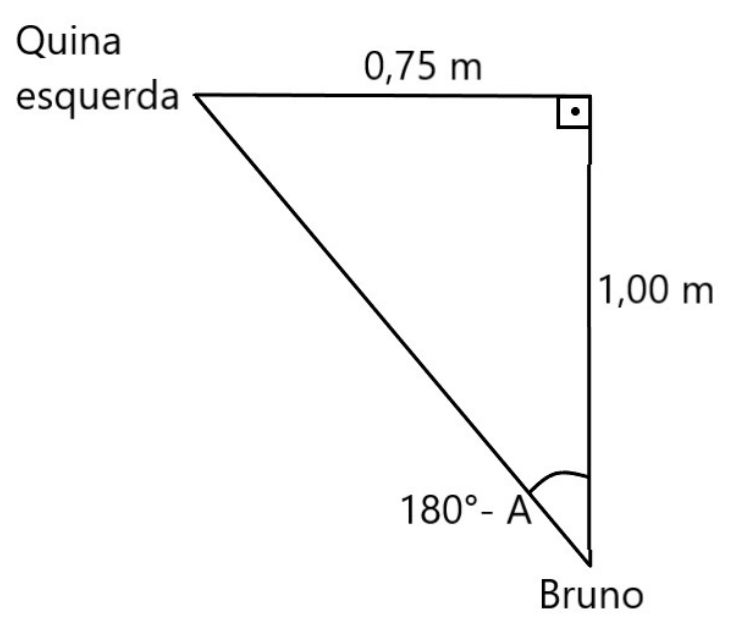
\includegraphics[width=0.6\linewidth]{imagens/tricima.png}
    \end{figure}

    \[A = 180^\circ - \tan^{-1}\left(\frac{0.75}{1.00}\right) = 143.1^\circ\]

    The hypotenuse of this triangle is \(\sqrt{0.75^2+1.00^2} = 1.25\text{m}\). That length will matter later.

    There are two possibilities for Shaula's coordinates. If Shaula rises east of the door, Bruno starts to see the star somewhere on the left side of the door. Otherwise, he starts to see Shaula somewhere on the horizon.

    The next step is therefore the azimuth at which Shaula rises. Apply a law of cosines in the PAZ triangle at $h=0$: 

    \[\cos A_0 = \frac{\sin\delta}{\cos\phi}\rightarrow A_0 = 128.7^\circ\]

    Since Shaula rises east of the door, Bruno can first see the star when it is exactly on the left side of the door. Shaula's $x$ coordinate is then the left side of the door ($x = 0$). When Bruno first sees it, Shaula's azimuth is $A=143.1^\circ$.

    Shaula's declination and azimuth are now known, as is the observer's latitude. Using the PAZ triangle again, 

    \[\cos h = \frac{\sin\phi\sin h - \sin \delta}{\cos\phi\cos A}\]

    Iteration gives \(h = 61.2^\circ\).

    The following right triangle gives the height difference between Bruno's eyes and Shaula's projection on the door:

    \begin{figure}[H]
        \centering
        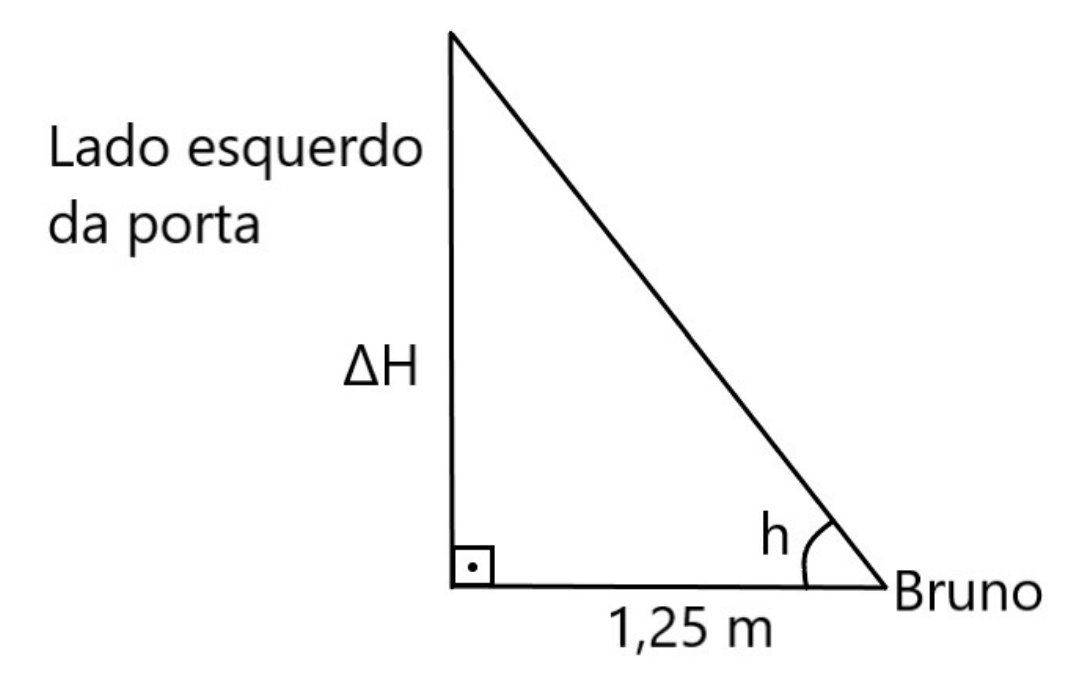
\includegraphics[width=0.6\linewidth]{imagens/tri1.png}
    \end{figure}

    The leg of \(1.25 \text{m}\) is the distance from Bruno to the left edge of the door found above.

    \[\Delta H = 1.25 \tan h = 2.27\text{m}\]

    Adding the height of Bruno's eyes gives the height of Shaula's projection on the door (the star's \(y\) coordinate):

    \[H_{\text{Shaula}} = H_{\text{eye}}+\Delta H \]

    \[H_{\text{Shaula}} = 3.47\text{m}\]

    So, when Bruno first sees Shaula that night, the star is at the \(\boxed{\text{point } (0, 3.47)}\) in the door's coordinate system.
\end{pssolution*}
\end{pproblem}

\end{document}
